\Aufgabe[e]{Dimensionierung eines Behälters}{
Finde das maximale Volumen eines kegelförmigen Trinkbechers, wenn die Mantellinie $R=1$ und $r$ und $h$ beliebig sind.

\begin{center}
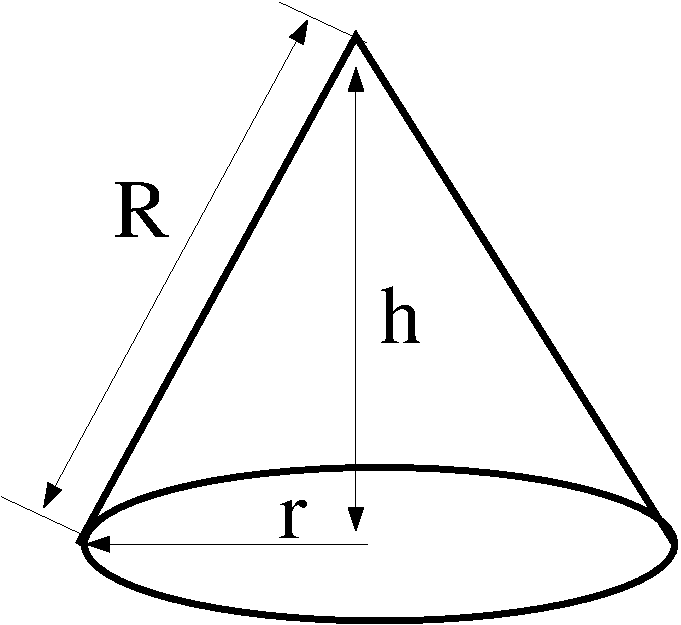
\includegraphics[width =0.2\textwidth]{../A/Wiederholung/cone.pdf}
\end{center}


Hinweis: Das Volume des Kegels ist $V = \frac13\, \pi\, r^2\, h$.
}

\Loesung{
Mit Pythagoras haben wir
$$
r^2 = R^2-h^2.
$$
Das Volumen des Kegels ist
$$
V(h) = \frac13 \pi (R^2-h^2)h = \frac13 \pi R^2 h - \frac13 \pi h^3.
$$
Das Maximum des Volumens findet man durch Untersuchung der kritischen Pukte der Funktion V. Die Nullstelle der Ableitung der Funktion $V$ ist
$$
V'(h) = \frac13 \pi R^2 - \pi h^2 = 0 \quad \Longrightarrow \quad h^2 = \frac13 R^2.
$$
Die zweite Ableitung ist stets negativ:
$$
V''(h) = -2\pi h < 0, \quad \forall h > 0,
$$
daher ist der kritische Punkt ein Maximum.
Aus der Beziehung $r^2 = R^2-h^2$ ist $r^2 = \frac23 R^2$.
Das maximale Volumen ist
$$
V = \frac13 \pi \frac23 R^2 \frac{1}{\sqrt{3}} R = \frac{2\pi}{9 \sqrt{3}} R^3.
$$
Für $R=1$ ist
$$
V = \frac{2\pi}{9 \sqrt{3}}.
$$

}


